\chapter{Gestione dei dispositivi di IO}
I dospositivi di input/output (o I/O), sono tutti quei dispositivi che si connettono alla classica architettura composta solo da processore e memoria centrale. Tra tali dispositivi rientrano: Memorie di massa (HDD e SSD), mouse, tastiera, sensori ecc.
Data l'eterogeneità di tali periferiche è richiesto che queste ultime siano gestite in un certo modo, o almeno, che la loro gestione principale sia di un certo tipo. Ciò, quindi, pone le basi su come dovremmo interfacciarci all'utilizzo di tali dispositivi

\section{Architettura generale di un dispositivo di I/O}
In generale un dispositivo di I/O può essere visto come l'insieme di tre parti fondamentali:
\begin{itemize}

    \item \textbf{Registri Dato, Stato e Controllo}: Tali registri sono quelli che interagiscono in maniera diretta con la CPU, e vengono utilizzati da quest'ultima per controllare e gestire le informazioni di quel dato dispositivo. Tali registri sono presenti internamente all'architattura del Calcolatore (ad esempio sulla scheda madre)

    \item \textbf{Sistema di adattamento}: Il sistema di adattamento adatta i segnali provenienti dal mondo esterno per essere letti o scritti nei registri di Dato, Stato e Controllo, e quindi permette di adattare l'attacco esterno (tipo l'USB che utilizza comunicazioni sequenziali), con la comunicazione parallela che il processore ha con i registri

    \item \textbf{Mondo esterno}: Per mondo esterno si intende tutta la parte che interagisce con il dispositivo in maniera fisica, ed il dispositivo fisico stesso. Quindi immaginiamoci anche una tastiera con il suo connettore USB

\end{itemize}

Un esempio di dispositivo esterno è la memoria HDD.
La memoria HDD ha difatti i tre registri di Dato, Stato e Controllo, quando si vuole scrivere su tale memoria, la CPU va a modificare i registri in modo da garantire tale operazione. Mentre la CPU modifica tali dati, il sistema di adattamento converte i dati presenti in quei tre registri in movimenti della testina + scrittura, rispettando sempre i controlli dati dalla CPU. La scrittura/lettura dei dati tramite la testina e la testina stessa rappresentano, invece, il mondo esterno.
Un altro esempio di periferica è la classica porta UART, che trasmette i sui dati in serie, ma il suo controllo avviene in parallelo. Pertanto al suo interno avrà sia un timer per scandire il clock in base alla tipologia di comunicazione, e poi avrà un buffer parallelo serie, che converte l'informazione da trasmettere in tanti bit seriali. Oltre alla parte parallelo-serie sarà anche dotato di una parte serie-parallelo, nel caso della ricezione.


\subsection{Modalità di comunicazione}
Le tipologie di collegamento che si possono avere tra un processore e le sue periferiche sono le seguenti:
\begin{itemize}
    \item \textbf{Collegamento passivo}: la periferica e la CPU non condividono alcun tipo di comunicazione. Quindi la CPU presuppone che la periferica sia sempre pronta ed è quindi solo lei a decidere quando e come utilizzare i dati, anche se questi magari non sono pronti o ben processati
    \item \textbf{Collegamento Sincrono}: La periferica e la CPU comunicano tra loro, la comunicazione è sincronizzata da un clock comune
    \item \textbf{Collegamento con Handshacking}: L'handshackin è una modalità di sincronizzazione asincrona, poichè si sfruttano dei segnali di comunicazione tra la CPU e la periferica che permettono di capire quando il dato è "pronto" o meno. Una classica implementazione è quella del segnale di req che viene alzato dal processore per far capire che vuole leggere e dall'ack emanato dalla periferica che fa comprendere che il dato è pronto o che è stata presa in carico l'operazione
    \item \textbf{Collegamento semisincrono}: Si condividono le stesse modalità di una comunicazione con handshacking, con la differenza che la sincronizzazione delle due parti avviene mediante uno stesso clock
\end{itemize}

\subsection{Interfacciamento CPU e periferica}
Per utilizzare le periferiche la CPU deve poter accedere ai registri di Dato, Stato e Controllo di tali periferiche. Le tipologie di interfacciamento che ci possono essere tra CPU e Periferica sono:
\begin{itemize}
    \item \textbf{Memory Mapped I/O}: La CPU fa riferimento ai registri di Dato, Stato e Controllo di una periferica come se fossero dei registri in memoria
    \item \textbf{I/O Mapped}: La CPU ha specifici comandi per interagire con le periferiche di I/O
\end{itemize}

Nel nostro caso il Motorola 68k è una tipologia di architettura memory mapped, e quindi la trattazione dei registri avviene mediante i classici comandi di spostamento già utilizzati

\subsubsection{Memory Mapped I/O}
Nel caso di interfacciamento con una struttura Memory Mapped, l'accesso ai registri di una determinata periferica avvengono tramite i bus di collegamento classici, che collegano anche la memoria ecc. Ciò quindi mi limita nell'utilizzo degli indirizzi, poichè, quando faccio riferimento ad un registro di una periferica, tale indirizzo non deve appartenere al set di indirizzi della memoria centrale

\subsubsection{I/O Mapped}
Nel caso di interfacciamento con una struttura I/O Mapped, l'accesso ai registri di una determinata periferica avviene mediante degli specifici comandi. Questo perchè le periferiche sono collegate a bus dedicati o hanno una gestione dedicata, che quindi differisce dalle comunicazioni che avvengono in generale all'interno dell'architettura al costo di avere meno modi di indirizzamento, dato che non si userà più la MOVE che è un codice operativo ortogonale

\subsubsection{Logiche di selezione}
Quando devo selezionare la mia periferica a cui faccio riferimento, utilizzo una serie di indirizzi. Tali indirizzi possono essere utili al fine di realizzare i seguenti tipi di logica:
\begin{itemize}
    \item \textbf{Logica tristate}: Logica che quando una periferica non vede il suo indirizzo sui bus adeguati smette di interagire con il sistema, quindi ignora la variazione dei dati sul bus. Tale logica, quindi utilizza l'indirizzo interno della nostra periferica
    \item \textbf{Logica Plug-and-play}: L'indirizzo della periferica viene scelto in base ad una serie di indirizzi disponibili
\end{itemize}

\subsection{BUS}
I bus sono i collegamenti che interconnettono le varie componenti di un calcolatore, ovvero, CPU, memoria e periferiche di I/O.
In generale non vi è una tipologia unica di bus, ve ne sono varie in base alla tipologia di utilizzi e alla tipologia di tecnologie utilizzate.
I bus, si contraddistinguono principalmente per la divisione che attuano sui loro collegamenti, ma in generale, le informazioni che vengono trasportate sono solitamente le stesse.
Le informazioni, quindi, sono dipartite tra i vari collegamenti presenti in un BUS. I collegamenti generici che si possono identificare in un bus sono:
\begin{itemize}
    \item \textbf{Alimentazione}: Collegamenti che principalmente comprendono la VCC (o più VCC), che sarebbero le tensioni di alimentazione delle componenti; ed il cavo di terra (o GND)
    \item \textbf{Dati}: Collegamenti che trasportano i dati che vengono interscambiati tra i vari dispositivi
    \item \textbf{Indirizzo}: Collegamenti che trasportano gli indirizzi che permettono la selezione dei dispositivi interessati o dei registri a cui si vuole accedere
    \item \textbf{Controllo}: Collegamenti che trasportano le informazioni inerenti alla tipologia di operazione che si vuole effettuare
    \item \textbf{Stato}: Collegamenti che permettono il controllo di flusso e la segnalazione di eventuali conflitti o errori
\end{itemize}

Data una tipologia di bus, può capitare che la periferica che vado ad utilizzare non è ad-hoc per quella determinata tipologia di bus. Pertanto, quello che posso fare, è considerare l'utilizzo di un \textbf{adapter}, che mi permette di adattare il bus classico con la tipologia di attacco specifica per la mia periferica. Oltretutto in alcuni casi, quando il dispositivo non permette la configurazione degli indirizzi, per evitare conflitti, l'adapter gestisce anche la gestione di tale indirizzo rispetto al sistema

\subsection{Driver}
I driver sono dei programmi che permettono di capire come il processore vada ad utilizzare una determinata periferica.
Le tipologie di approccio che si possono avere nella scrittura dei driver sono varie, la più primitiva è il polling.
Il \textbf{Polling} è un modo con cui il processore va ad interagire con la periferica. In generale si va a dare un primo segnale di controllo alla periferica e si aspetta uno specifico valore di stato per poter accedere al dato. Tali sistema è altamente inefficiente, poichè mentre la CPU aspetta la riposta della periferica passano dei periodi di clock dove la CPU rimane ferma. Il tempo che quindi la CPU rimane senza eseguire delle operazioni utili è detto \textbf{Busy-waiting}. Un possibile codice di implementazione del polling è [\ref{m68:polling}]

\begin{lstlisting}[caption={Codice polling}, label=m68:polling]
        ORG      $8000
*Inizializzo lo stato dei miei registri
        MOVE.B   #$00,C
        MOVE.B   #$00,S
*Vado a considerare la zona di memoria dove voglio salvare i dati
        MOVEA.L  #VAR1,A0
        MOVE.W  #0,D0
*Devo prelevare N dati quindi ciclo N volte
FOR     CMP.W   #N,D0
        BGE   FUORI

*Qui devo scrivere il driver sapendo  che devo ricevere un byte

        MOVE.B  #$01,C  *Vado a settare un controllo
*Qui inizia il ciclo di polling dove attendo uno specifico valore dello stato
L1      MOVE.B  S,D1
        AND.B  #$80,D1  *Se il bit si e' alzato ho finito. Altrimenti continuo ad aspettare
        BEQ  L1

*Qui il dato e' stato letto, poiche' ho il flag di stato alzato
        MOVE.B  D,(A0)+ *Inserisco il dato in memoria
        MOVE.B  #$00,C  *Vado a resettare il segnale di Controllo
        MOVE.B  #$00,S  *Vado ad "eludere" il sistema su un segnale di stato

FUORI   ADD.B  #1,D0             *Incremento il conteggio
        BRA  FOR                 *Ripeti

        ORG     $8100
D       DS.B    1   *Registro dato
S       DS.B    1   *Registro Stato
C       DS.B    1   *Registro Controllo

N       EQU     5   *Quantita' di valori da considerare
VAR1    DS.B    5   *Array effettivo di raccolta dati
\end{lstlisting}
\newpage
Il codice [\ref{m68:polling}] presenta però le seguenti criticità:
\begin{itemize}
    \item \textbf{Mancata Generalizzazione}: Si vanno a considerare in maniera diretta i registri in memoria D,S e C. Che per l'implmentazione di un driver riutilizzabile non è proprio la scelta corretta
    \item \textbf{Polling}: L'attesa che viene svolta all'interno di tale codice non permette al processore di eseguire altri passi prima di aver ricevuto tutti i caratteri
    \item \textbf{Gestione dei malfunzionamenti}: Se la periferica ha un qualunque tipo di malfunzionamento e quindi non aggiorna mai il registro di stato, tale ciclo eseguirà all'infinito senza mai fermarsi
\end{itemize}

Le due problematiche (o criticità), possono essere affrontate in vario modo. Per la prima la soluzione è molto semplice, al posto di andare a considerare i registri di Dato, Stato e Controllo in maniera diretta, possono essere considerati come registri indirizzo (Ai), a cui vado ad associare gli indirizzi di tali registri. Tali inidirizzi poi vengono settati secondo un determinato criterio prima della chiamata al driver.
Per ovviare, invece, al secondo problema c'è il bisogno di considerare le \textbf{interruzioni}. Mentre per l'ultimo problema la soluzione è l'introduzione di \textbf{timer}, che permettono di capire quando un sistema sta impiegando un tempo più grande del dovuto per eseguire un operazione, ciò permette di poter gestire ed uscire da situazioni di eventuali guasti.

\subsubsection{Interruzioni}
L'interruzione è un evento che cambia la normale esecuzione di un programma per fargli eseguire prima del codice specifico per la gestione di quella determinata condizione [\ref{img:bootint}]. In generale non è corretto parlare solo di interruzioni, poichè tale termine non comprende o non può comprendere anche il caso in cui le interruzioni vengano scatenate dall'interno per casistiche particolari. Difatti è più corretto fare la seguente suddivisione:
\begin{itemize}
    \item \textbf{Interruzioni}: Segnali che sono a contatto con le periferiche e che permettono alla CPU di interrompersi e di eseguire il codice per la gestione della comunicazione con quella data interfaccia. Le interruzioni sono scatenate, quindi, dal dispositivo che vuole interagire con la CPU
    \item \textbf{Eccezioni}: Funzionano come le interruzioni, con la differenza che vengono scatenate internamente rispetto al processore, quindi non vengono gestite dai dispositivi ma dal programma stesso, tale condizione fa eseguire comunque una ISR, con l'obbiettivo di dover gestire particolari casistiche (es. divisione per 0)
\end{itemize}

\begin{figure}
    \centering
    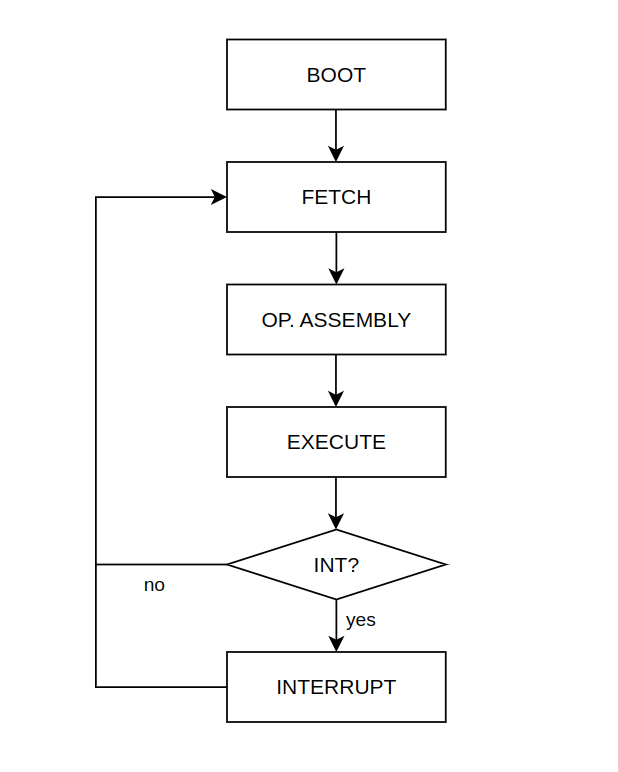
\includegraphics[width=0.5\textwidth]{img/BootInt.png}
    \caption{Ciclo di esecuizone con interrupt}\label{img:bootint}
\end{figure}
Quindi quando le interruzioni sono scatenate vanno ad effettuare una chiamata a subroutine particolare, tale chiamata è detta ISR (Interrupt-Services-Routine). Tale situazione, quindi, ferma il sistema dalla sua normale esecuzione del programma per dare priorità alla gestione dell'interruzione. Questo, quindi, apre molti dubbi su come gestire lo stato in cui si trova la macchina, poichè se quando torno dalla ISR, ho cambiato qualche registro significativo si potrebbe compromettere il normale funzionamento del programma. In generale i due registri che richiedono l'obbligo di essere salvari sono i registri: \textbf{SR(Status register)} e il \textbf{PC(Program Counter)}. In generale, i registri che vado a salvare in questo passaggio sono anche detti: \textbf{Descrittore di processo}, tali registri, quindi, descrivono lo stato di funzionamento del mio processore quando poi è stato prelazionato dalla mia ISR. Ciò mi permette di proseguire ancora con la normale esecuzione del programma prefissato.

\subsubsection{Gestione delle Interruzioni}
Una volta definito cosa sono le interruzioni è di fondamentale importanza capire come il processore le gestisce. Le principali modalità di gestione delle interruzioni sono due e sono:
\begin{itemize}
    \item \textbf{Vettorizzate}: Ogni livello di priorità di interrupt è collegato al processore. I fili di collegamento per le interrupt sono limitati, quindi più dispositivi possono collegarsi sullo stesso cavo di interrupt. Il processore, quindi, per identificare il dispositivo che ha scatenato l'Interrupt va a controllare i bus, su cui il dispositivo ha caricato il suo codice identificativo. Identificare il dispositivo, vuol dire identificare la tipologia di ISR da andare ad utilizzare. Gli indirizzi degli entry-point delle varie periferiche sono memorizzati in memoria a partire dall'indirizzo 0 a seguire per 256 locazioni di 4 byte. Tali locazioni si dividono nel seguente modo:
    \begin{itemize}
        \item \textbf{Funzioni speciali}: Da 0 a 24, gli entry-point identificano delle funzioni speciali o di gestione aritmentica
        \item \textbf{Interruzioni autovettorizzate}: da 25 a 31 sono indicizzate le locazioni per il funzionamento autovettorizzato
        \item \textbf{Trap}: da 32 a 47 sono indicizzate le funzioni per la gestione dei Trap
        \item \textbf{Utilizzabili}: da 48 a 256 sono locazioni disponibili per l'inserimento degli entry-point per la gestione di diverse periferiche
    \end{itemize}
    \item \textbf{Autovattorizzate}: A differenza del caso vettorizzato, evita la lettura del codice identificativo, poichè ogni livello di interrupt è collegato al vettore delle ISR autovettorizzate e permette di selezionare in maniera "ignorante" l'ISR alla locazione della tipologia di priorità inserita
\end{itemize}

\subsubsection{PIC} \label{par:PIC}
In generale, nel caso di sistema \textbf{vettorizzato}, viene in aiuto il componente \textbf{PIC (Programmable Interrupt Controller)} [\ref{img:PIC}].
Il PIC è un dispositivo che permette di arricchire le
modalità di gestione delle interruzioni. Grazie alla programmazione di questo oggetto, possiamo assegnare alle varie periferiche non una sola linea di interruzione con una specifica ISR, ma possiamo esplorare tutto il vettore delle interruzioni, che in teoria è costituito da 256 locazioni. In sostanza, il PIC permette di usare interrupt vettorizzate, ovvero il dispositivo fornisce sul data bus un vettore di 8 bit che rappresenta l’indice all’interno della tabella delle interruzioni corrispondente all’indirizzo della corretta ISR. Nel M68k questo protocollo è simulato con il PIC: Il dispositivo non scrive sul data bus il vettore di 8 bit, ma comunica l’interruzione al PIC che si occuperà di capire qual è il vettore corrispondente al dispositivo interrotto. Il PIC estende la gestione delle interruzioni del processore M68K introducendo nuove funzionalità, come la gestione prioritaria, la mascheratura delle interruzioni e le linee di interrupt. Il dispositivo ha in uscita verso il processore una linea di interruzione INT e una linea di INTA (acknowledgement) , mentre ha in ingresso 8 linee di interruzioni differenti, a priorità decrescente (0 massima, 7 minima). Più dispositivi possono essere connessi in cascata, fino a 8 per un massimo di 64 linee di interruzione.
Il PIC accetta richieste di interruzione dai dispositivi di IO connessi alle sue linee e determina, a seconda dell’algoritmo di gestione prioritaria selezionato, quale delle interruzioni simultaneamente attiva ha la priorità più alta. Dopodiché trasmette un segnale sulla linea INT al processore, attende un segnale su INTA (handshaking) e poi trasmette sul bus dati il vettore di 8 bit a cui corrisponde la corretta interruzione sulla tabella delle interruzioni.
Il Control Register interno al PIC permette di configurare la gestione prioritaria mediante un’opportuna modifica:
\begin{itemize}
    \item \textbf{Fully nested}: le richieste di interruzione sono ordinate secondo uno schema a priorità fissa che va da IR0 a IR7;
    \item \textbf{Round Robin}: Schema prioritario a rotazione, ovvero la linea di interruzione più prioritaria appena servita diventa la meno prioritaria dopo il servizio;
    \item \textbf{Maschera interruzioni} consente l’inibizione o l’abilitazione delle linee di interruzione.
\end{itemize}

Il modo di operazione scelto dev essere configurato in fase di inizializzazione del PIC, ma può anche essere dinamicamente cambianto da un apposito programma di gestione.
L’Interrupt Request Register (IRR) riceve in ingresso le 8 linee di interruzione provenienti dalle periferiche collegate e ne memorizza lo stato. L’input a questo registro è gestito da un circuito integrato che si occupa della gestione prioritaria delle interruzioni, mentre l’output è il registro In Service Register (ISR) in cui vengono memorizzati solo i segnali di interruzione da servire in accordo alla maschera (IMR). Il Type Register (TR) è un registro di 8 bit che memorizza nei 5 bit più significativi il valore base del vettore da scrivere in output sul bus dati, mentre nei 3 meno significativi uno spiazzamento in accordo alla linea interrompente. Dopo il servizio, l’i-esimo bit di IRR è automaticamente cancellato per riuovere la causa di interruzione.

\begin{figure}
    \centering
    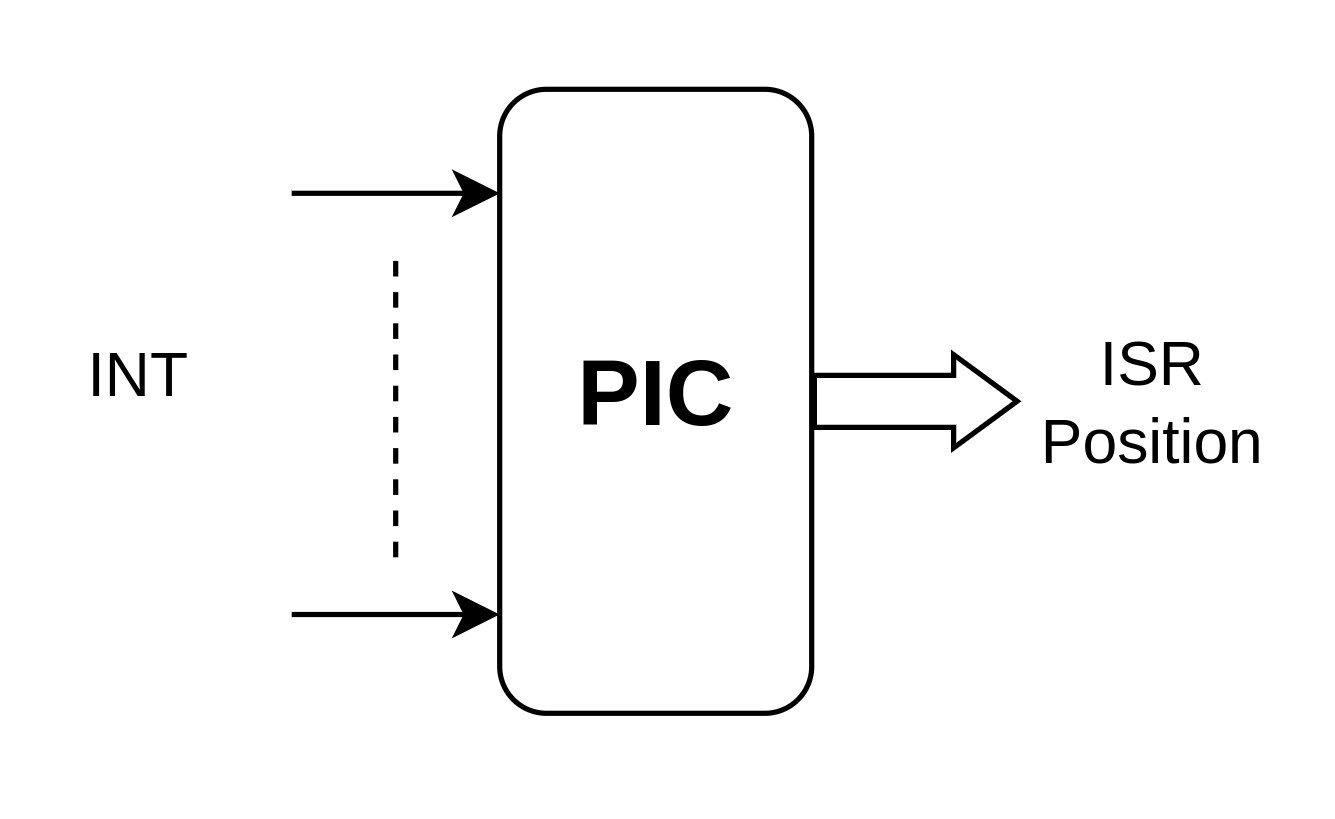
\includegraphics[width=0.7\textwidth]{img/PIC.png}
    \caption{PIC(Programmable Interrupt Controller)}\label{img:PIC}
\end{figure}

\begin{figure}
    \centering
    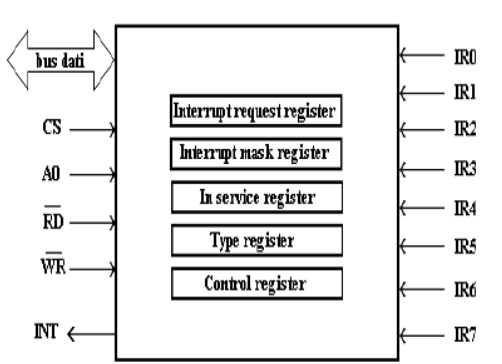
\includegraphics[width=0.5\textwidth]{img/PIC2.png}
    \caption{PIC: modello di programmazione}\label{img:PIC2}
\end{figure}


\subsection{Estensione del modello IO generale}
Un modello di architettura dotato solo di PIA (\ref{par:PIA}) è limitato: può gestire solo caratteri, ha a disposizione solo 7 interruzioni e può generare attese infinite con il protocollo di handshaking.
Per risolvere questi problemi, vengono introdotti nuovi elementi nell'architettura: \textbf{DMA} per gestire il trasferimento di messaggi invece di caratteri, \textbf{PIC} (\ref{par:PIC}) per superare la limitazione sul numero di ISR indirizzabili e \textbf{TIMER} per gestire la temporizzazione e il risolvere il problema delle attese infinite (\ref{img:IO_ESTESO}).

\begin{figure}[!ht]
    \centering
    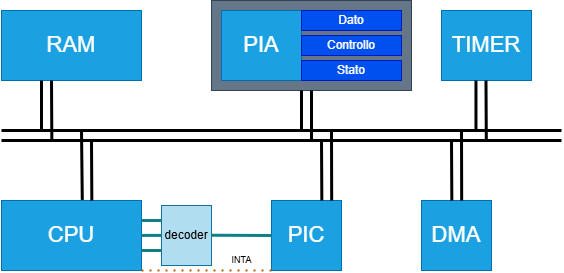
\includegraphics[width=0.75\textwidth]{img/Schema_IO_1.png}
    \caption{Modello IO esteso - schema logico}
    \label{img:IO_ESTESO}
\end{figure}

Il timer espone il modello di programmazione Registro di stato, Registro di valore e Registro di Modo. Nel registro di valore di solito è scritto un istante in cui il timer si "sveglia" e genera un'interruzione: infatti il timer possiede una linea con la quale può comunicare un'interruzione.

\section{DMA (Direct Memory Access)}\label{par:DMA}

Il \textbf{DMA} è un dispositivo che permette di sollevare il processore dall'onere di trasferire i dati tra varie periferiche. Questo significa che i dispositivi possono comunicare direttamente con la memoria senza passare per la CPU. In particolare, il DMA permette di gestire il trasferimento dati tra:
\begin{itemize}
    \item \textbf{Memoria $\leftrightarrow$ Periferica};
    \item \textbf{Periferica $\leftrightarrow$ Memoria};
    \item \textbf{Memoria $\leftrightarrow$ Memoria}.
\end{itemize}

Il suo principio di funzionamento è semplice, ed è schematizzabile tramite tre registri principali:
\begin{itemize}
    \item \textbf{Registro Indirizzo}: indica l'indirizzo da cui prelevare il dato;
    \item \textbf{Registro Conteggio}: indica il conteggio del numero di dati trasferiti e permette di capire quando interrompere il trasferimento;
    \item \textbf{Registro Identificativo}: tramite tale registro si identifica:
    \begin{itemize}
        \item o il dispositivo da considerare per il trasferimento;
        \item o l'area di memoria da considerare per il trasferimento.
    \end{itemize}  
\end{itemize}

La reale architettura del DMA è però più complessa. La maggior complessità dell'architettura proviene da varie problematiche che si possono riscontrare durante il funzionamento, come, ad esempio, l'accesso al BUS dati in maniera concorrente al processore. \uppercase{È} pertanto necessario che il DMA non sia collegato al processore solo tramite il bus dati, ma anche tramite vari segnali di controllo, che permettono al processore e al DMA di potersi coordinare.

Il dispositivo di riferimento nelle esercitazioni del corso è l'\textbf{Intel 8237}, che per la sua architettura dispone di 4 canali per il collegamento con 4 dispositivi diversi. Nella versione simulata in ASIM, tale componente è composto di soli 2 canali.

Scendendo più nei dettagli, il dispositivo reale è in grado di sostenere 4 modalità di funzionamento differenti:
\begin{itemize}
    \item \textbf{Single}: si trasferisce una \textit{word} alla volta; dopo aver trasferito una word, il DMA restituisce il BUS al processore almeno per un ciclo;
    \item \textbf{Block}: si trasferisce un intero \textit{blocco} non appena il DMA acquisisce il BUS. Alla fine del trasferimento viene inoltrata un'interruzione al processore che segnala la disponibilità del BUS;
    \item \textbf{On Demand}: simile alla modalità Block, con la differenza che il trasferimento può essere interrotto dal processore e poi ripreso, grazie ai registri contatore, dall'esatto punto in cui era stato interrotto;
    \item \textbf{Cascade}: modalità di funzionamento che permette di collegare più DMA in cascata per gestire più di 4 canali.
\end{itemize}

Il DMA acquisisce il controllo del bus attraverso il seguente processo (fare riferimento alla figura \ref{img:architettura-dma}):
\begin{itemize}
    \item IL DMA richiede il possesso del bus al processore tramite il segnale BR Bus Request;
    \item Il processore fornisce il consenso alla richiesta di utilizzo del bus tramite il segnale BG Bus Grant;
    \item Il dispositivo che ha richiesto il bus fornisce l'ack al processore mediante il segnale BGACK, e il processore viene scollegato elettricamente dal BUS indirizzi.
\end{itemize}
Il DMA si interfaccia con le periferiche mediante i segnali DREQ e DACK: DREQ è una richiesta da parte della periferica per il DMA di un trasferimento dati, mentre DACK è la comunicazione da parte del DMA che un dispositivo è stato selezionato per un trasferimento, ed è propagato una volta che il DAC ha acquisito l'accesso al bus indirizzi.


Oltre al minor numero di canali, il componente simulato in ASIM non supporta tutte le modalità sopra citate: le modalità utilizzabili in ASIM sono infatti \textbf{Single} e \textbf{Block}.

Guardando la figura~\ref{img:DMA}, abbiamo il modello architetturale del componente realizzato in ASIM, in cui i registri posti sulla sinistra sono di comunicazione con il processore, mentre i segnali sulla destra servono per l'interfacciamento con le periferiche collegate ai canali.

Per la comunicazione con il processore, i segnali rappresentati hanno il seguente significato:
\begin{itemize}
    \item \textbf{D0-D7}: collegamento al BUS dati da e verso il componente;
    \item $\overline{\mathbf{CS}}$: segnale binario di selezione del dispositivo;
    \item \textbf{A0-A3}: attenzione! Non tutti i segnali $A_i$, ma solo i 4 meno significativi, vengono utilizzati per la selezione dello specifico registro interno;
    \item $\overline{\mathbf{IOR}}$ e $\overline{\mathbf{IOW}}$: segnali di gestione della lettura e della scrittura sul componente e sulle periferiche;
    \item $\overline{\mathbf{MEMR}}$ e $\overline{\mathbf{MEMW}}$: segnali di gestione della lettura e della scrittura sui dispositivi di memoria;
    \item \textbf{CLK e Reset}: classici segnali di clock (tempificazione) e reset dei registri del dispositivo;
    \item \textbf{HRQ}: segnale di richiesta del controllo del sistema BUS, solitamente collegato all'ingresso HOLD della CPU;
    \item \textbf{HLDA}: segnale proveniente dalla CPU che segnala l'acquisizione del BUS da parte del processore;
    \item $\overline{\mathbf{EOP}}$: linea di interruzione \textit{bidirezionale} che si collega al processore per segnalare il completamento del trasferimento.
\end{itemize}

Dati i due differenti canali, si avranno due periferiche collegate allo stesso dispositivo DMA. La comunicazione può essere effettuata da una sola periferica per volta. Tale decisione è presa secondo un ordine di priorità, per cui il dispositivo collegato ai terminali 0 ha priorità maggiore rispetto a quello collegato ai terminali 1. I segnali che gestiscono le periferiche sono:

\begin{itemize}
    \item \textbf{DREQ0 e DREQ1}: segnali usati dalle periferiche per richiedere l'accesso al BUS tramite cicli DMA;
    \item \textbf{DACK0 e DACK1}: segnali con cui il DMA comunica alla periferica la disponibilità a soddisfare la richiesta.
\end{itemize}

\begin{figure}[ht]
    \centering
    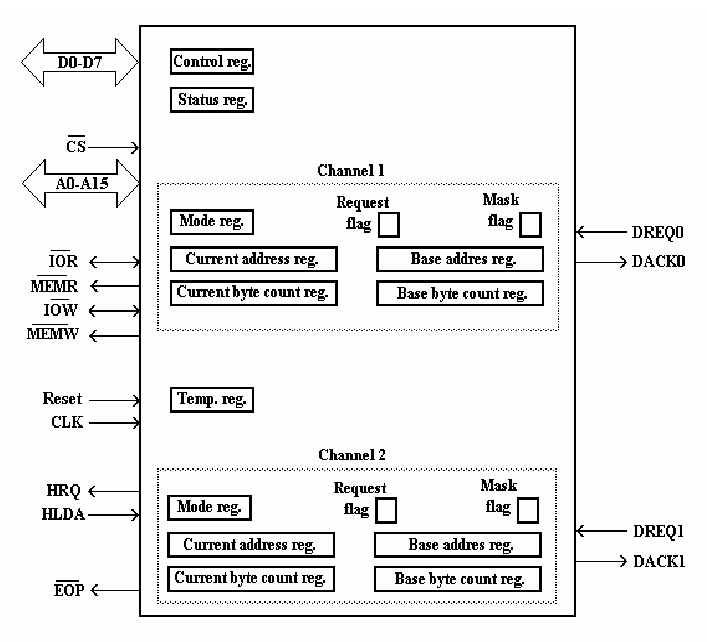
\includegraphics[width=.7\textwidth]{img/DMA.png}
    \caption{Modello di programmazione DMA a 2 canali}
    \label{img:DMA}
\end{figure}

Consideriamo il canale 0 del DMA, ed analizziamo il modello di programmazione.
Il registro CADDR0 (Current Adress) contiene l'indirizzo della locazione di memoria interessata dal trasferimento, ed è accessibile in lettura e scrittura all'indirizzo relativo \$0. Il registro BADDR0 (Base Address) contiene l'indirizzo iniziale di CADDR0, ed è accessibile in scrittura automaticamente insieme a CADDR0. 
Il registro CCOUNT0 (Current Count) contiene il numero attuale di byte da trasferire, ed è accessibile in lettura e scrittura all'indirizzo relativo \$1. Il registro BCOUNT0 (Base Count) contiene il numero di byte iniziale da trasferire, ed è accessibile in scrittura automaticamente insieme a CCOUNT0. Il registro MODE0 contiene informazioni sul modo di funzionamento del canale 0, ed è accessibile in scrittura all'indirizzo relativo \$B. Il Control Register è unico, e i suoi 8 bit sono suddivisi nei 4 meno significativi che indicano lo stato del componente, mentre i 4 più significativi sono bit di controllo. \uppercase{è} accessibile sia in scrittura che in lettura all'indirizzo relativo \$8.
All'indirizzo relativo \$9 è accessibile in sola scrittura il flag RF (REQUEST FLAG), che è il flag dove segnalare una richiesta da software al DMA per un trasferimento, ed è del tutto analogo di una richiesta da periferica tramite segnali appositi; la selezione del canale avviene sul bit meno significativo del dato scritto nel registro (*******0 per il canale 0, *******1 per il canale 1) mentre il valore che si vuole assegnare al flag deve essere scritto sul quarto bit del dato (\%00001000 $\rightarrow$ \$08 $\rightarrow$ RF alto sul canale 0). MF Mask Flag, accessibile in sola scrittura all'indirizzo relativo \$A, serve a mascherare con il valore alto le richieste dei rispettivi canali.  


\subsection{Utilizzo effettivo in ASIM}

Per capire come utilizzare il DMA, occorre prima stabilire cosa il DMA dovrà fare e in che modo lavorerà. Per definire queste cose si usano i registri di controllo (unico per tutti i canali) e i registri di Modo (uno per ogni canale). Quando si dichiara il componente nel file di configurazione, si definiscono due indirizzi (address 1 e address 2) che individuano sedici locazioni accessibili dal processore come registri di memoria (\textit{memory mapped}). Il decodificatore collegato sul pin $\overline{\mathbf{CS}}$ attiva il pin quando rileva sul bus indirizzi un valore compreso nell'insieme [address1, address2].

All'interno del file di configurazione vi sono anche le altre voci che identificano come il componente si collega ai vari BUS e agli altri oggetti del sistema. Una buona rappresentazione logica del sistema DMA si trova nella figura~\ref{img:architettura-dma}.

\begin{figure}[ht]
    \centering
    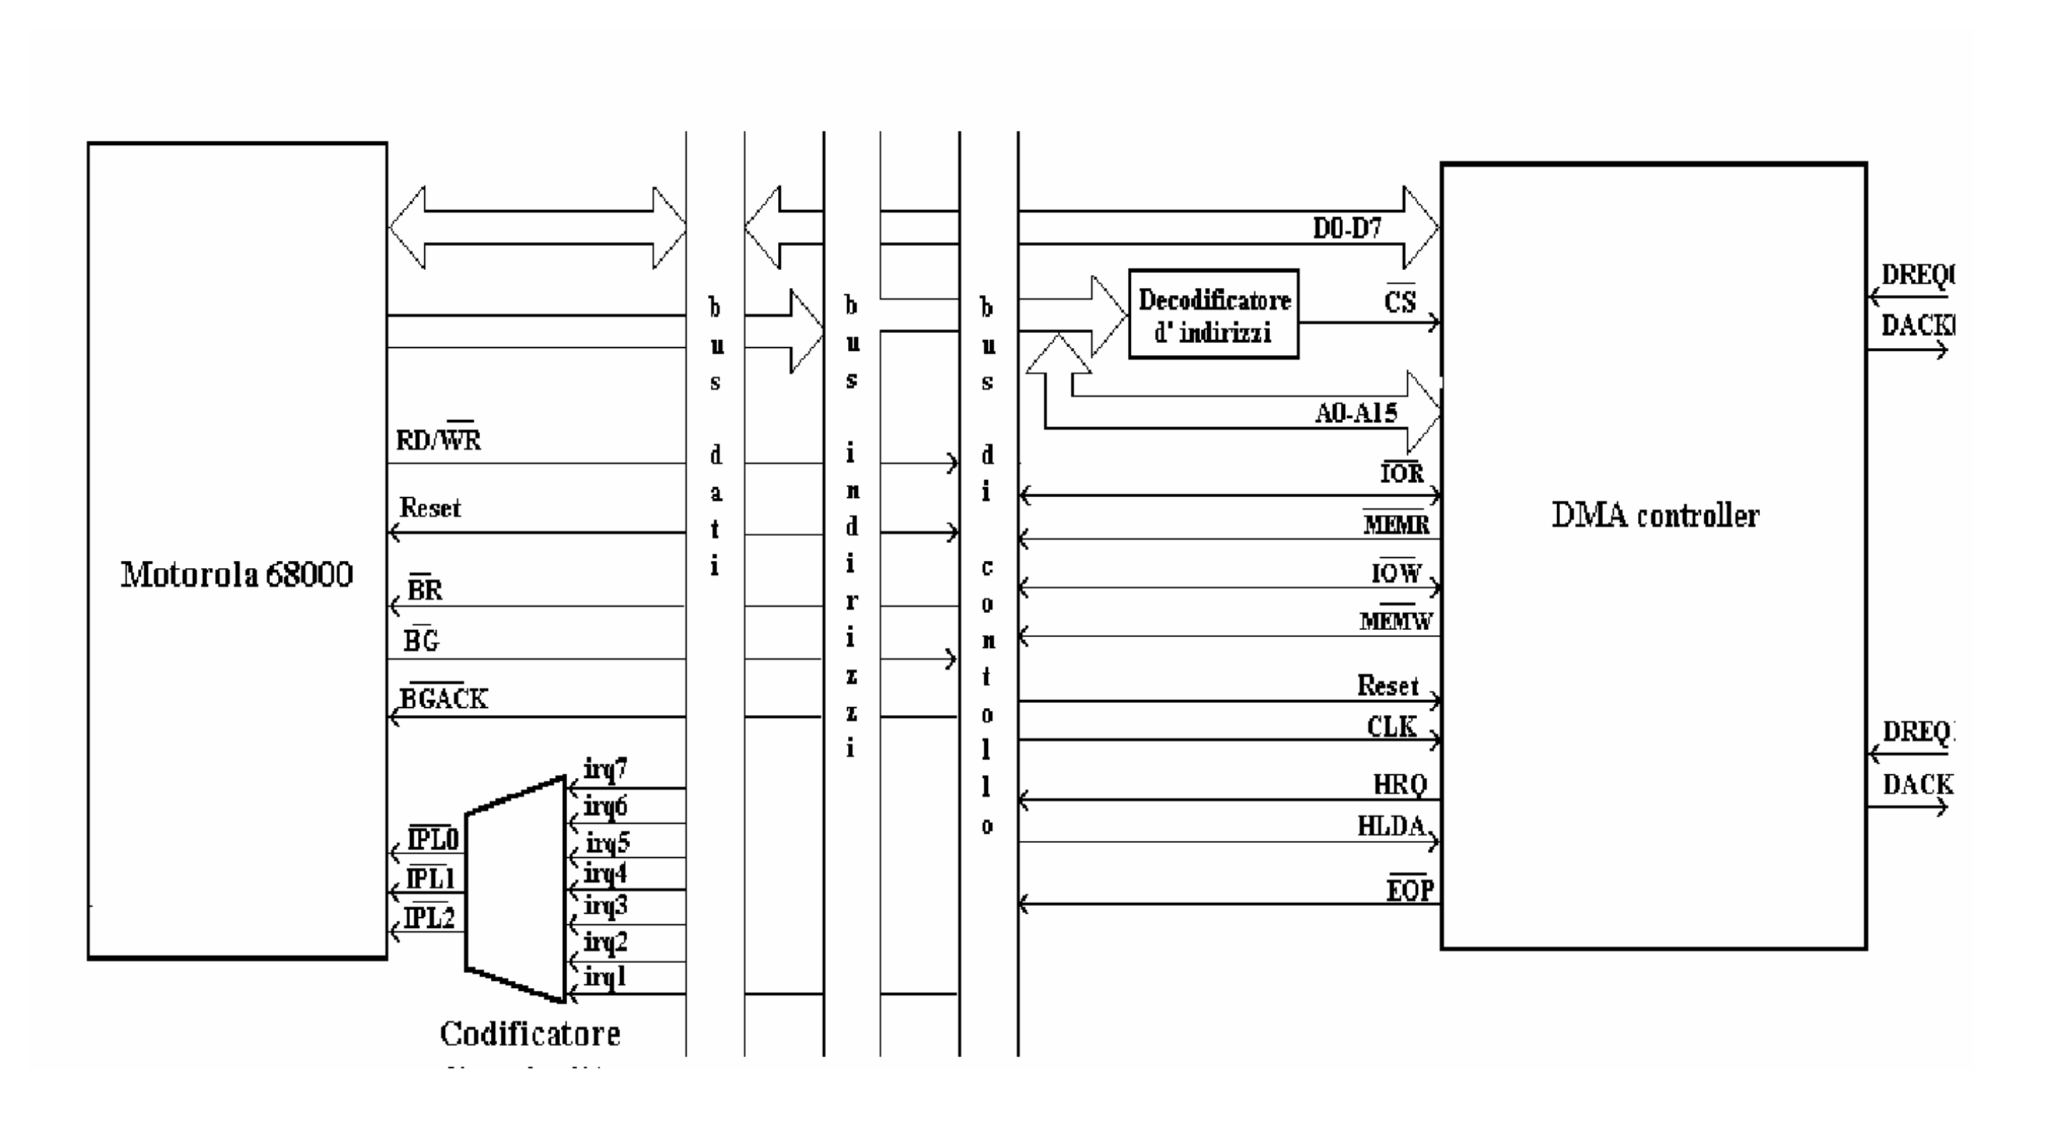
\includegraphics[width=.7\textwidth]{img/architettura-dma.png}
    \caption{Montaggio del componente DMA rispetto al sistema generale}
    \label{img:architettura-dma}
\end{figure}

Una volta compresa l'architettura del sistema, possiamo analizzare il significato dei bit dei vari registri interni.

\paragraph{Registro Mode}
Il registro Mode (uno per canale) è descritto nella Tabella~\ref{tab:MODE-8237}.
\begin{table}[ht]
    \centering
    \begin{tabular}{|c|p{11cm}|}
    \hline
    \textbf{Bit} & \textbf{Significato} \\ \hline
    0 & Instrada il dato su un canale: 0 per il canale 0, 1 per il canale 1 \\ \hline
    1-2 & Non utilizzati \\ \hline
    3 & Direzione di trasferimento: 0 = da memoria a interfaccia, 1 = da interfaccia a memoria \\ \hline
    4 & Abilita l'\textbf{Autoinizializzazione}: se impostato a 1, alla fine del conteggio resetta i registri con i valori di base \\ \hline
    5 & Incremento di CADDR (0) o decremento (1) \\ \hline
    6 & Non utilizzato \\ \hline
    7 & Modalità di trasferimento: 0 = Single, 1 = Block \\ \hline
    \end{tabular}
    \caption{Significato dei bit del registro MODE}
    \label{tab:MODE-8237}
\end{table}

\paragraph{Registro di Controllo}
Il registro di controllo del DMA controller è illustrato nella Tabella~\ref{tab:CTRL-8237}.
\begin{table}[ht]
    \centering
    \begin{tabular}{|c|p{11cm}|}
    \hline
    \textbf{Bit} & \textbf{Significato} \\ \hline
    0 & Termina conteggio per il canale 0 \\ \hline
    1 & Termina conteggio per il canale 1 \\ \hline
    2 & È stata inoltrata una richiesta al canale 0 \\ \hline
    3 & È stata inoltrata una richiesta al canale 1 \\ \hline
    4 & Non utilizzato \\ \hline
    5 & Abilita il trasferimento da memoria a memoria \\ \hline
    6 & Impone che in un trasferimento memoria-memoria l'indirizzo sorgente rimanga costante \\ \hline
    7 & Abilita il DMA controller \\ \hline
    \end{tabular}
    \caption{Significato dei bit del registro CTRL}
    \label{tab:CTRL-8237}
\end{table}

\newpage

\subsection{Implementazione in Motorola 68k}

Le implementazioni in ASIM con Motorola 68k sfruttano varie architetture definite nei file di configurazione. Una volta definita l'architettura, si stabilisce come gestire i registri e le periferiche (come il DMA). 

\subsubsection{Caso Memoria-Memoria}

Nel caso memoria-memoria, il DMA richiede una particolare definizione. Si devono definire:
\begin{itemize}
    \item l'area dati (origine e destinazione);
    \item gli intervalli per l'accesso ai registri interni del DMA.
\end{itemize}

\begin{lstlisting}
                ORG     $9500
origine         DC.B    0,1,2,3,4,5,6,7,8,9 * msg
destinazione    DS.B    34

* Definizione di indirizzo e offset per accesso ai registri DMA
dma             EQU     $2010
caddr0          EQU     0
caddr1          EQU     2
ccount1         EQU     3
cntrl           EQU     8
mode            EQU     11
reset           EQU     13
clearmf         EQU     14
writeamf        EQU     15
nbyte           EQU     34
\end{lstlisting}

Una volta definita la parte "statica", si passa alla parte operativa:

\begin{lstlisting}
    ORG         $8200 

    MOVE.W      #dma,A0           * Carico l'indirizzo del DMA

* Carico l'indirizzo di origine dei dati nel primo registro indirizzo
    MOVE.W      #origine,caddr0(A0)

* Carico l'indirizzo di destinazione nel secondo registro indirizzo
    MOVE.W      #destinazione,caddr1(A0)

* Numero di caratteri da trasferire
    MOVE.B      #nbyte,ccount1(A0)

* Configuro il primo canale: Block, incremento, autoinizializzazione
    MOVE.B      #$90,mode(A0)

* Configuro il secondo canale in modo analogo
    MOVE.B      #$91,mode(A0)

* Set del control register
    MOVE.B      #$A0,cntrl(A0)

* Ciclo caldo
LOOP    JMP     LOOP
\end{lstlisting}

Alla fine del trasferimento, occorre gestire l'interruzione scatenata. L'ISR ha come scopo il reset del DMA:

\begin{lstlisting}
        ORG     $8700

int7    MOVE.L  A0,-(A7)           * Salva il contesto
        MOVE.W  #dma,A0
        MOVE.B  #0,reset(A0)       * Resetta il DMA
        MOVE.L  (A7)+,A0           * Ripristina il registro
        RTE
\end{lstlisting}

\subsubsection{Caso Dispositivo $\rightarrow$ Memoria}
La configurazione che studiamo in questo paragrafo rappresenta due sistemi in comunicazione, uno in trasmissione e uno in ricezione tramite due PIA. La PIA in trasmissione manda continuamente caratteri alla PIA in ricezione, il DMA collegato al sistema in ricezione sposta i caratteri ricevuti dalla PIA verso la Memoria, senza passare per il processore. 
Presentiamo innanzitutto il sistema in trasmissione che denominiamo S1, che effettua il trasferimento con un semplice ciclo.

\begin{lstlisting}
***AREA DATI***
        ORG     $8000
MSG     DC.B    1,2,3,4,5,6
DIM     DC.B    6

***MAIN***
        ORG     $8200
PIADB   EQU     $2006
PIACB   EQU     $2007 


MAIN    JSR     DVBOUT 
        MOVEA.L #PIACB,A1 
        MOVEA.L #PIADB,A2 
        MOVEA.L #MSG,A0 
        MOVE.B  DIM,D0
        CLR     D1
        MOVE    D0,D2 
INVIO   MOVE.B  (A0)+,D1 
        MOVE.B  D1,(A2) 
        ADDQ    #-1,D2
        BNE     INVIO 

LOOP    JMP     LOOP 

DVBOUT  MOVE.B  #0,PIACB
        MOVE.B  #$FF,PIADB 
        MOVE.B  #%00100100
        RTS 
\end{lstlisting}

Osserviamo che in questo caso non effettuiamo l'handshaking, e non effettuiamo la lettura fittizia per assicurarci che CRB7 sia basso, semplciemente scriviamo sul PRB. Questo è dovuto al fatto che il DMA non possiede segnali per parlare direttamente con la PIA, quindi \textit{forziamo} una scrittura senza handshaking.
Procediamo con la presentazione del driver di un sistema che riceve un messaggio di 30 caratteri su una PIA e lo copia in memoria direttamente tramite un DMA. Assumiamo che la PIA sia collegata al canale 0 del DMA e che la linea di interruzione del DMA sia collegata sulla linea 7 del processore (Autovettore 31).

\begin{lstlisting}
***AREA DATI***
PIADA   EQU     $2004
PIACA   EQU     $2005

dma     EQU     $2010 
caddr0  EQU     0
ccount0 EQU     1
cntrl   EQU     8
request EQU     9
mode0   EQU     11
nbyte   EQU     30


        ORG     $8000
msg     DS.B    nbyte 

***AREA CODICE***
        ORG     $8200
MAIN    JSR     DVAIN 
        MOVE.W  SR,D0 
        ANDI.W  #$D8FF,D0 *stato utente, int abilitate 
        MOVE.W  D0,SR 

        MOVE.W  dma,A1 
        MOVE.B  #nbyte,ccount0(A1)
        MOVE.W  msg,caddr0(A1)
        MOVE    #$08,mode0(A1)
        MOVE    #$80,cntrl(A1)
        MOVE    #$08,request(A1)

LOOP    JUMP    LOOP 

DVAIN   MOVE    #0,PIACA
        MOVE.W  #00,PIADA 
        MOVE    #$00100101,PIACA 
        RTS 

**ISR FINE TRASFERIMENTO*** 
        ORG     $8700
        NOP 
        RTE 


\end{lstlisting}

\subsubsection{Caso Memoria $\rightarrow$ Dispositivo}
In questo caso, un dispositivo  deve trasmettere un messaggio da un'area di memoria verso una PIA usando il DMA. La PIA deve essere programmata per ricevere dati, quindi il porto va configurato in INPUT. Nell'esempio presentato a lezione, non si affronta la questione del trasferimento da PIA del sistema S1 a PIA del sistema S2, quindi il programma non funziona ed è presentato al solo scopo didattico di illustrare il passaggio da Memoria e Interfaccia dispositivo tramite DMA. 

\begin{lstlisting}
***AREA COSTANTI***
PIADA   EQU     $2004
PIACA   EQU     $2005

dma     EQU     $2010
caddr0  EQU     0
ccount0 EQU     1
cntrol  EQU     8
request EQU     9
mode0   EQU     11
nbyte   EQU     6

***AREA DATI*** 
        ORG     $8000
MSG     DC.B    1,2,3,4,5,6
DIM     DC.B    6

***AREA CODICE***
MAIN    JSR     PIAINIT
        MOVE.W  SR,D0 
        ANDI.W  #$D8FF,D0
        MOVE.W  D0,SR 

        MOVE.W  #dma,A1 
        MOVE.W  #nbyte,ccount0(A1)
        MOVE.W  #msg,caddr0(A1)
        MOVE    #$10000000,mode0(A1)
        MOVE    #$08,request(A1)

LOOP    JMP     LOOP 

PIAINIT MOVE    #0,PIACA 
        MOVE    #$00,PIADA 
        MOVE    #%00100100,PIACA 
        RTS 

\end{lstlisting}
